\documentclass{article}
\usepackage[utf8]{inputenc}


% Language setting
% Replace `english' with e.g. `spanish' to change the document language
\usepackage[spanish]{babel}

% Set page size and margins
% Replace `letterpaper' with `a4paper' for UK/EU standard size
\usepackage[letterpaper,top=2cm,bottom=2cm,left=3cm,right=3cm,marginparwidth=1.75cm]{geometry}

% Useful packages
\usepackage{amsmath}
\usepackage{graphicx}
\usepackage[colorlinks=true, allcolors=blue]{hyperref}
\usepackage{amsthm}
\usepackage{amssymb}
\PassOptionsToPackage{normalem}{ulem}
\usepackage{ulem}
\usepackage[T1]{fontenc}
\usepackage{float}
\usepackage{xmpmulti}
\usepackage{algorithm,algpseudocode}
\usepackage{amsmath}
\usepackage{tabularx}

\title{Proyecto taquin Análisis de Algoritmos}
\author{Camilo Hernández Guerrero\\Samy Felipe Cuestas Merchán\\Juan Camilo Mendieta Hernández}

\begin{document}

\maketitle

\section{Parte I: Análisis y diseño del algoritmo}
\subsection{Análisis}
El problema consiste en crear un jugador automático para Taquín el cual es un juego que consiste en mover cuadrículas de una unidad con una figura o numeros en una matriz cuadrada hasta ordenar la figura o la secuencia de números.
Se abordará este problema con un método eurístico donde se calcularán los posibles tableros dependiendo de cada jugada realizada, donde la probabilidad de ganar se calcula a partir de la distancia euclidiana que tiene el tablero actual con el tablero que ya está resuelto, buscando una ruta que de una posible solución. Debido a la gran cantidad de posibles caminos que pueden deribar de una jugada, una solución de fuerza bruta no es adecuada.

\subsection{Diseño}
Usando el análisis previo se sabe que para resolver el problema del jugador automatico de Taquín, se van a necesitar para el diseño del algoritmo en los componentes de las entradas y las salidas los siguientes datos para cada función a usar.

\subsubsection{Verificar tablero}
\begin{itemize}
    \item Entrada
    \\Se necesita la matriz del tablero de juego actual y la matriz del tablero resuelto.
    \item Salida
    \\Un valor booleano indicando si se gano el juego.
\end{itemize}

\subsubsection{Moverse hacia arriba, abajo, derecha e izquierda}
\begin{itemize}
    \item Entrada
    \\Se necesita la matriz del tablero de juego actual y las coordenadas del espacio en blanco.
    \item Salida
    \\Coordenas de la nueva ubicación del espacio en blanco.
\end{itemize}

\subsubsection{Euristica}
\begin{itemize}
    \item Entrada
    \\Se necesita el numero de de movimientos que se han realizado y la distancia euclidiana para resolver el tablero.
    \item Salida
    \\Número que representa la medida de la eurística.
\end{itemize}

\subsubsection{Buscar posición de un elemento}
\begin{itemize}
    \item Entrada
    \\Se necesita la matriz del tablero actual y el elemento a buscar en la matriz.
    \item Salida
    \\Coordenas en la matriz donde se ubica el elemento.
\end{itemize}

\subsubsection{Calcular distancia euclidiana}
\begin{itemize}
    \item Entrada
    \\Se necesita la matriz del tablero de juego actual y la matriz del tablero resuelto.
    \item Salida
    \\Numero con el calculo de la distancia euclidiana.
\end{itemize}

\subsubsection{Obtener posibles movimientos}
\begin{itemize}
    \item Entrada
    \\Se necesita la matriz del tablero de juego actua, la matriz del tablero resuelto y un nodo del arbol con los tableros posibles
    \item Salida
    \\Listado de movimientos que se pueden hacer.
\end{itemize}

\subsubsection{Buscar mejor nodo}
\begin{itemize}
    \item Entrada
    \\Listado con posibles tableros para jugar
    \item Salida
    \\Nodo con un tablero que tiene la menor distancia con el tablero completado.
\end{itemize}

\subsubsection{Movimiento automático}
\begin{itemize}
    \item Entrada
    \\Se necesita la matriz del tablero actual y la matriz con el table resuelto.
    \item Salida
    \\Listado de los movimientos a realizar para ganar.
\end{itemize}

\subsubsection{Inicializar tablero}
\begin{itemize}
    \item Entrada
    \\Numero para generar la matriz cuadrada.
    \item Salida
    \\Una matriz con objetos desoredenados para empezar el juego.
\end{itemize}

\section{Parte II: Pseudocódigo}
\begin{algorithm}[H]
\begin{algorithmic}[1]
\Procedure{gameWon}{$table, tableWon, n$}
  \State{$result \leftarrow true$}
  \For{$row \leftarrow0$ \textbf{to} $n$}
    \For{$column\leftarrow0$ \textbf{to} $n$}
      \If{$table[row][column] \neq tableWon[row][column]$}
        \State{$result \leftarrow false$}
      \EndIf
    \EndFor
  \EndFor
  \State\Return{$result$}
\EndProcedure
\end{algorithmic}
\caption{Función que verifica si ganó el juego}
\end{algorithm}

\begin{algorithm}[H]
\begin{algorithmic}[1]
\Procedure{moveUp}{$table, blankSpace$}
  \If{$blankSpace[0] \neq 0$}
    \State{$aux \leftarrow table[blankSpace[0]-1][blankSpace[1]]$}
    \State{$table[blankSpace[0]-1][blankSpace[1]] \leftarrow " "$}
    \State{$table[blankSpace[0]][blankSpace[1]] \leftarrow aux$}
    \State{$blankSpace \leftarrow (blankSpace[0] - 1, blankSpace[1])$}
    \State\Return{$blankSpace$}
  \Else
    \State\Return{$blankSpace$}
  \EndIf
\EndProcedure
\end{algorithmic}
\caption{Función que mueve la pieza hacia arriba}
\end{algorithm}

\begin{algorithm}[H]
\begin{algorithmic}[1]
\Procedure{moveDown}{$table, blankSpace$}
  \If{$blankSpace[0] < \left|table[0]\right| - 1$}
    \State{$aux \leftarrow table[blankSpace[0] + 1][blankSpace[1]]$}
    \State{$table[blankSpace[0] + 1][blankSpace[1]] \leftarrow " "$}
    \State{$table[blankSpace[0]][blankSpace[1]] \leftarrow aux$}
    \State{$blankSpace \leftarrow (blankSpace[0] + 1, blankSpace[1])$}
    \State\Return{$blankSpace$}
  \Else
    \State\Return{$blankSpace$}
  \EndIf
\EndProcedure
\end{algorithmic}
\caption{Función que mueve la pieza hacia abajo}
\end{algorithm}

\begin{algorithm}[H]
\begin{algorithmic}[1]
\Procedure{moveLeft}{$table, blankSpace$}
  \If{$blankSpace[1] > 0$}
    \State{$aux \leftarrow table[blankSpace[0]][blankSpace[1]-1]$}
    \State{$table [blankSpace[0]][blankSpace[1]-1] \leftarrow " "$}
    \State{$table [blankSpace[0]][blankSpace[1]] \leftarrow aux$}
    \State{$blankSpace \leftarrow (blankSpace[0] , blankSpace[1] - 1)$}
    \State\Return{$blankSpace$}
  \Else
    \State\Return{$blankSpace$}
  \EndIf
\EndProcedure
\end{algorithmic}
\caption{Función que mueve la pieza hacia la izquierda}
\end{algorithm}

\begin{algorithm}[H]
\begin{algorithmic}[1]
\Procedure{moveRight}{$table, blankSpace$}
  \If{$blankSpace[1] < \left|table[0]\right| - 1$}
    \State{$aux \leftarrow table[blankSpace[0] ][blankSpace[1] + 1]$}
    \State{$table [blankSpace[0] ][blankSpace[1] + 1] \leftarrow " "$}
    \State{$table [blankSpace[0]][blankSpace[1]] \leftarrow aux$}
    \State{$blankSpace \leftarrow (blankSpace[0] , blankSpace[1] + 1)$}
    \State\Return{$blankSpace$}
  \Else
    \State\Return{$blankSpace$}
  \EndIf
\EndProcedure
\end{algorithmic}
\caption{Función que mueve la pieza hacia la derecha}
\end{algorithm}

\begin{algorithm}[H]
\begin{algorithmic}[1]
\Procedure{getElementPosition}{$currentPuzzleTable, element$}
  \For{$i \leftarrow0$ \textbf{to} $\left|currentPuzzleTable\right|$}
    \If{$element in currentPuzzleTable[i]$}
      \State\Return{$(i, currentPuzzleTable[i].index(element))$}
    \EndIf
  \EndFor
\EndProcedure
\end{algorithmic}
\caption{Función que obtiene la posición del elemento}
\end{algorithm}

\begin{algorithm}[H]
\begin{algorithmic}[1]
\Procedure{tableEuclidianDistance}{$currentPuzzleTable, tableWon$}
  \State{$tableDistance \leftarrow 0$}
  \For{$i \leftarrow0$ \textbf{to} $\left|currentPuzzleTable\right|$}
    \For{$j \leftarrow0$ \textbf{to} $\left|currentPuzzleTable\right|$}
      \State{$positionTableWon \leftarrow getElementPosition(tableWon, currentPuzzleTable[i][j])$}
      \State{$tableDistance \leftarrow tableDistance + ABS(i - positionTableWon[0]) + ABS(j - positionTableWon[1])$}
    \EndFor
  \EndFor
  \State\Return{$tableDistance$}
\EndProcedure
\end{algorithmic}
\caption{Función que obtiene distancia euclidiana entre tablas}
\end{algorithm}

\begin{algorithm}[H]
\begin{algorithmic}[1]
\Procedure{getPossibleMoves}{$node, currentPuzzleTable, tableWon$}
  \State{$listOfMoves \leftarrow \emptyset$}
  \State{$blankCoordinates \leftarrow getElementPosition(node.currentPuzzleTable, " ")$}
  \State{$sizeCurrentPuzzle \leftarrow \left|currentPuzzleTable\right|$}
  \State{$newPosition \leftarrow (blankCoordinates[0] - 1, blankCoordinates[1])$}
  \If{$0 \leq newPosition[0] < sizeCurrentPuzzle$ \textbf{and} $0 \leq newPosition[1] < sizeCurrentPuzzle$}
    \State{$newPuzzleTable \leftarrow deepcopy(node.currentPuzzleTable)$}
    \State{$newPuzzleTable[blankCoordinates[0]][blankCoordinates[1]] \leftarrow node.currentPuzzleTable[newPosition[0]][newPosition[1]]$}
    \State{$newPuzzleTable[newPosition[0]][newPosition[1]] \leftarrow " "$}
    \State{$listOfMoves \leftarrow listOfMoves \cup Node(newPuzzleTable, node.currentPuzzleTable, node.numberOfMoves + 1, tableEuclidianDistance(currentPuzzleTable, tableWon),"U")$}
  \EndIf
  \State{$newPosition \leftarrow (blankCoordinates[0] + 1, blankCoordinates[1])$}
    \If{$0 \leq newPosition[0] < sizeCurrentPuzzle$ \textbf{and} $0 \leq newPosition[1] < sizeCurrentPuzzle$}
      \State{$newPuzzleTable \leftarrow deepcopy(node.currentPuzzleTable)$}
      \State{$newPuzzleTable[blankCoordinates[0]][blankCoordinates[1]] \leftarrow node.currentPuzzleTable[newPosition[0]][newPosition[1]]$}
      \State{$newPuzzleTable[newPosition[0]][newPosition[1]] \leftarrow " "$}
      \State{$listOfMoves \leftarrow listOfMoves \cup Node(newPuzzleTable, node.currentPuzzleTable, node.numberOfMoves + 1, tableEuclidianDistance(currentPuzzleTable, tableWon),"D")$}
    \EndIf
  \State{$newPosition \leftarrow (blankCoordinates[0] , blankCoordinates[1] + 1)$}
    \If{$0 \leq newPosition[0] < sizeCurrentPuzzle$ \textbf{and} $0 \leq newPosition[1] < sizeCurrentPuzzle$}
      \State{$newPuzzleTable \leftarrow deepcopy(node.currentPuzzleTable)$}
      \State{$newPuzzleTable[blankCoordinates[0]][blankCoordinates[1]] \leftarrow node.currentPuzzleTable[newPosition[0]][newPosition[1]]$}
      \State{$newPuzzleTable[newPosition[0]][newPosition[1]] \leftarrow " "$}
      \State{$listOfMoves \leftarrow listOfMoves \cup Node(newPuzzleTable, node.currentPuzzleTable, node.numberOfMoves + 1, tableEuclidianDistance(currentPuzzleTable, tableWon),"R")$}
    \EndIf
  \State{$newPosition \leftarrow (blankCoordinates[0] , blankCoordinates[1] - 1)$}
    \If{$0 \leq newPosition[0] < sizeCurrentPuzzle$ \textbf{and} $0 \leq newPosition[1] < sizeCurrentPuzzle$}
      \State{$newPuzzleTable \leftarrow deepcopy(node.currentPuzzleTable)$}
      \State{$newPuzzleTable[blankCoordinates[0]][blankCoordinates[1]] \leftarrow node.currentPuzzleTable[newPosition[0]][newPosition[1]]$}
      \State{$newPuzzleTable[newPosition[0]][newPosition[1]] \leftarrow " "$}
      \State{$listOfMoves \leftarrow listOfMoves \cup Node(newPuzzleTable, node.currentPuzzleTable, node.numberOfMoves + 1, tableEuclidianDistance(currentPuzzleTable, tableWon),"L")$}
    \EndIf
  \State\Return{$listOfMoves$}
\EndProcedure
\end{algorithmic}
\caption{Función que retorna los movimientos posibles}
\end{algorithm}

\begin{algorithm}[H]
\begin{algorithmic}[1]
\Procedure{getBestNode}{$dictionaryOfNodes$}
  \State{$i \leftarrow 0$}
  \State{$bestEuristic \leftarrow \infty$}
  \For{$node \leftarrow 0$ \textbf{to} $dictionaryOfNodes.values()$}
    \If{$i = 0$ \textbf{or} $node.euristic() < bestEuristic$}
      \State{$i \leftarrow i + i + 1$}
      \State{$bestNode \leftarrow node$}
      \State{$bestEuristic \leftarrow bestNode.euristic()$}
    \EndIf
  \EndFor
  \State\Return{$bestNode$}
\EndProcedure
\end{algorithmic}
\caption{Función que obtiene el mejor nodo}
\end{algorithm}

\begin{algorithm}[H]
\begin{algorithmic}[1]
\Procedure{movement}{$actualTable, tableWon$}
  \State{$moves \leftarrow {str(actualTable): Node(actualTable, actualTable, 0, tableEuclidianDistance(actualTable, tableWon), "")}$}
  \State{$movesToWin \leftarrow \emptyset$}
  \While{$true$}
    \State{$testMove \leftarrow getBestNode(moves)$}
    \State{$movesToWin[str(testMove.currentPuzzleTable)] \leftarrow testMove$}
    \If{$testMove.currentPuzzleTable = tableWon$}
        \State{$auxNode \leftarrow movesToWin[str(tableWon)]$}
        \State{$auxMoves \leftarrow list()$}
        \While{auxNode.direction}
            \State{$auxMoves \leftarrow auxMoves \cup auxNode.direction as direction, auxNode.currentPuzzle Table as node$}
            \State{$auxNode \leftarrow movesToWin[str(auxNode.previousPuzzleTable)]$}
        \EndWhile
        \State{$auxMoves.reverse()$}
        \State\Return{$auxMoves$}
    \EndIf
    \State{$possibleMoves \leftarrow getPossibleMoves(testMove,actualTable, tableWon)$}
    \For{$node \leftarrow 0$ \textbf{to} $\left|possibleMoves\right|$}
        \If{$str(node.currentPuzzleTable) in movesToWin.keys()$ \textbf{or} $str(node.currentPuzzleTable) in moves.keys()$ \textbf{and} $moves[str(node.currentPuzzleTable)].euristic() < node.euristic()$}
            \State{\textbf{continue}}
        \EndIf
        \State{$moves[str(node.currentPuzzleTable)] \leftarrow node$}
    \EndFor
    \State{\textbf{delete} $ moves[str(testMove.currentPuzzleTable)]$}
  \EndWhile
\EndProcedure
\end{algorithmic}
\caption{Función de movimiento}
\end{algorithm}

\begin{algorithm}[H]
\begin{algorithmic}[1]
\Procedure{slicePuzzle}{ }
  \State{$n \leftarrow 3$}
  \State{$randomPuzzle \leftarrow \emptyset$}
  \State{$puzzle \leftarrow \emptyset$}
  \State{$puzzleWon \leftarrow \emptyset$}
  \State{$let numbersInOrder[0..(n*n)] be a sequence.$}
  \State{$let numbersWithoutOrder[0..(n*n)] be a random sequence.$}
  \State{$blank \leftarrow (0, 0)$}
  \State{$i \leftarrow 0$}
  \For{$numberA \leftarrow 0$ \textbf{to} $n$}
    \State{$aux \leftarrow \emptyset$}
      \For{$numberB \leftarrow 0$ \textbf{to} $n$}
        \If{$numbersWithoutOrder[i] \neq (n*n)-1$}
          \State{$aux \leftarrow aux \cup str(numbersWithoutOrder[i])$}
        \Else
          \State{$aux \leftarrow aux \cup " "$}
          \State{$blank \leftarrow (numberA, numberB)$}
        \EndIf
        \State{$i \leftarrow i + 1$}
      \EndFor
      \State{$randomPuzzle \leftarrow randomPuzzle \cup aux$}
  \EndFor
  \State{$i \leftarrow 0$}
  \For{$numberA \leftarrow 0$ \textbf{to} $n$}
    \State{$aux \leftarrow \emptyset$}
      \For{$numberB \leftarrow 0$ \textbf{to} $n$}
        \If{$numbersInOrder[i] \neq (n*n)-1$}
          \State{$aux \leftarrow aux \cup str(numbersInOrder[i])$}
        \Else
          \State{$aux \leftarrow aux \cup " "$}
          \State{$blank \leftarrow (numberA, numberB)$}
        \EndIf
        \State{$i \leftarrow i + 1$}
      \EndFor
      \State{$puzzleWon \leftarrow puzzleWon \cup aux$}
  \EndFor
  \State{$puzzle \leftarrow randomPuzzle$}
  \State{$blank \leftarrow getElementPosition(puzzle, " ")$}
  \State{$movimientos \leftarrow movement(puzzle, puzzleWon)$}
  \State{$turn \leftarrow 0$}
  \While{$gameWon(puzzle, puzzleWon) = False$}
    \State{$command \leftarrow movimientos[turn]["direction"]$}
    \State{$turn \leftarrow turn + 1$}
    \If{$command = "U"$}
      \State{$blank \leftarrow moveUp(puzzle, blank)$}
    \ElsIf{$command = "D"$}
      \State{$blank \leftarrow moveDown(puzzle,blank)$}
    \ElsIf{$command = "L"$}
      \State{$blank \leftarrow moveLeft(puzzle,blank)$}
    \ElsIf{$command = "R"$}
      \State{$blank \leftarrow moveRight(puzzle,blank)$}
    \EndIf
  \EndWhile
  \State{\textbf{print} $puzzle$ \textbf{as Matrix}}
\EndProcedure
\end{algorithmic}
\caption{Función principal}
\end{algorithm}

\section{Parte III: Análisis de complejidad}
\subsection{Verificar tablero}
La complejidad de esta función es de O(n^2) debido a sus dos ciclos.
\subsection{Moverse hacia arriba, abajo, derecha e izquierda}
La complejidad de estas funciones es de O(1) debido a su falta de ciclos.
\subsection{Euristica}
\subsection{Buscar posición de un elemento}
La complejidad de esta función es de O(n) debido a su unico ciclo.
\subsection{Calcular distancia euclidiana}
La complejidad de esta función es de O(n^2) debido a sus dos ciclos.
\subsection{Obtener posibles movimientos}
La complejidad de estas funciones es de O(1) debido a su falta de ciclos.
\subsection{Buscar mejor nodo}
La complejidad de esta función es de O(n^2) debido a sus dos ciclos.
\subsection{Inicilizar tablero}
La complejidad de esta función es de O(n^2) debido a sus dos ciclos.

\section{Parte IV: Pruebas}
Para realizar las pruebas se utilizaron distintos tableros, aumentando la dificultad respecto a la cantidad de movimientos (turnos) necesaria teóricamente para resolver el tablero. Específicamente se evaluaron ocho tableros que difieren de dificiltad.
    \subsection{Tablero 3x3 resuelto en tres movimientos}
        \begin{figure}[H]
        \centering
        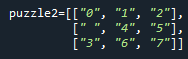
\includegraphics[width=0.3\textwidth]{puzzles/puzzle.PNG}
        \caption{Tablero 3x3 fácil sin resolver}
        \label{fig:ger}
        \end{figure}
        
        \begin{figure}[H]
        \centering
        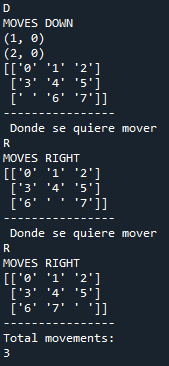
\includegraphics[width=0.3\textwidth]{puzzles/puzzleSolved.PNG}
        \caption{Tablero 3x3 fácil resuelto}
        \label{fig:ger}
        \end{figure}
    
    \subsection{Tablero 3x3 resuelto en doce movimientos}
        \begin{figure}[H]
        \centering
        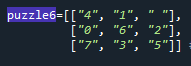
\includegraphics[width=0.3\textwidth]{puzzles/puzzle2.PNG}
        \caption{Segundo tablero 3x3 fácil sin resolver}
        \label{fig:ger}
        \end{figure}
        
        \begin{figure}[H]
        \centering
        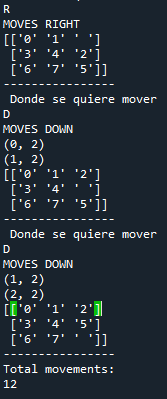
\includegraphics[width=0.3\textwidth]{puzzles/puzzle2Solved.PNG}
        \caption{Segundo tablero 3x3 fácil resuelto}
        \label{fig:ger}
        \end{figure}
        
    \subsection{Tablero 3x3 resuelto en catorce movimientos}
        \begin{figure}[H]
        \centering
        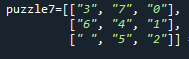
\includegraphics[width=0.3\textwidth]{puzzles/puzzle3.PNG}
        \caption{Tercer tablero 3x3 fácil sin resolver}
        \label{fig:ger}
        \end{figure}
        
        \begin{figure}[H]
        \centering
        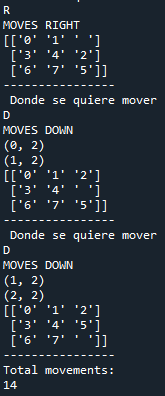
\includegraphics[width=0.3\textwidth]{puzzles/puzzle3Solved.PNG}
        \caption{Tercer tablero 3x3 fácil resuelto}
        \label{fig:ger}
        \end{figure}
        
    \subsection{Tablero 3x3 resuelto en dieciocho movimientos}
    Desde este tablero en adelante, los tableros empiezan a tardar considerablemente más, este tardó treinta y dos segundos en completarse utilizando como CPU un Intel i5 9600K corriendo a 4.6Ghz, cabe resaltar que los anteriores tableros no tardaban ni un segundo en resolverse.
        \begin{figure}[H]
        \centering
        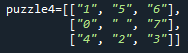
\includegraphics[width=0.3\textwidth]{puzzles/puzzle4.PNG}
        \caption{Cuarto tablero 3x3 sin resolver}
        \label{fig:ger}
        \end{figure}
        
        \begin{figure}[H]
        \centering
        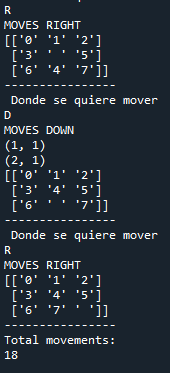
\includegraphics[width=0.3\textwidth]{puzzles/puzzle4Solved.PNG}
        \caption{Cuarto tablero 3x3 resuelto}
        \label{fig:ger}
        \end{figure}
        
    \subsection{Tablero 3x3 resuelto en veinte movimientos}
    Este tablero tardó en completarse dos minutos, cuarenta y ocho segundos.
        \begin{figure}[H]
        \centering
        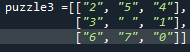
\includegraphics[width=0.3\textwidth]{puzzles/puzzle5.PNG}
        \caption{Quinto tablero 3x3 sin resolver}
        \label{fig:ger}
        \end{figure}
        
        \begin{figure}[H]
        \centering
        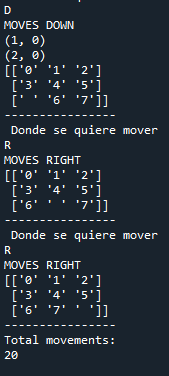
\includegraphics[width=0.3\textwidth]{puzzles/puzzle5Solved.PNG}
        \caption{Quinto tablero 3x3 resuelto}
        \label{fig:ger}
        \end{figure}
        
    \subsection{Tablero 3x3 resuelto en veintidos movimientos}
    Este tablero tardó en completarse cuatro minutos y treinta segundos.
        \begin{figure}[H]
        \centering
        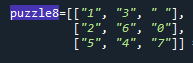
\includegraphics[width=0.3\textwidth]{puzzles/puzzle6.PNG}
        \caption{Sexto tablero 3x3 sin resolver}
        \label{fig:ger}
        \end{figure}
        
        \begin{figure}[H]
        \centering
        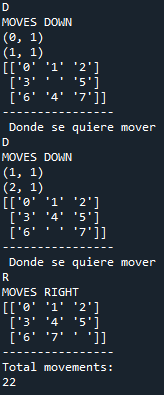
\includegraphics[width=0.3\textwidth]{puzzles/puzzle6Solved.PNG}
        \caption{Sexto tablero 3x3 resuelto}
        \label{fig:ger}
        \end{figure}
        
    \subsection{Tablero 3x3 resuelto en veinticuatro movimientos}
    Este tablero tardó en completarse diez minutos y diez segundos.
        \begin{figure}[H]
        \centering
        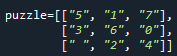
\includegraphics[width=0.3\textwidth]{puzzles/puzzle7.PNG}
        \caption{Séptimo tablero 3x3 difícil sin resolver}
        \label{fig:ger}
        \end{figure}
        
        \begin{figure}[H]
        \centering
        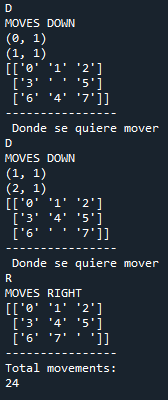
\includegraphics[width=0.3\textwidth]{puzzles/puzzle7Solved.PNG}
        \caption{Séptimo tablero 3x3 difícil resuelto}
        \label{fig:ger}
        \end{figure}
        
    \subsection{Tablero 4x4 resuelto en trece movimientos}
    Este tablero tardó en completarse cuarenta y siete segundos.
        \begin{figure}[H]
        \centering
        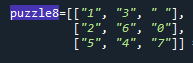
\includegraphics[width=0.3\textwidth]{puzzles/puzzle6.PNG}
        \caption{Tablero 4x4 sin resolver}
        \label{fig:ger}
        \end{figure}
        
        \begin{figure}[H]
        \centering
        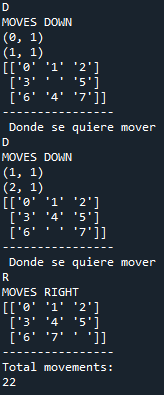
\includegraphics[width=0.3\textwidth]{puzzles/puzzle6Solved.PNG}
        \caption{Tablero 4x4 resuelto}
        \label{fig:ger}
        \end{figure}
        
\section{Parte V: Conclusión}
Para este proyecto el análisis previo del problema que se realizó fue muy importante ya que nos dio indicaciones del camino a seguir para desarrollar un algoritmo que funcionara, ya que en un inicio no se tenía muy claro como abordar la gran cantidad de opciones implicadas en la resolución del tablero de taquin, gracias a este analisis se pudo determinar que el mejor camino para resolver este problema era un algoritmo euristico, y se selecciono el algoritmo A* como inspiración para enfrentar el problema. 
Una vez finalizado el algoritmo A* para resolver el tablero de taquin se pudo comprobar que aunque si cumplía con este objetivo, las pruebas mostraban que en varios casos el tiempo que tardaba en resolverse un tablero era demasiado alto. Se pudo determinar con diferentes pruebas que esto se debe probablemente a un error en la forma en que se le da un peso a una opción por encima de otra, que es el mecanismo con el cual el algoritmo encuentra una solución, ya que en lugar de intentar todas las posibles opciones de movimiento, se prueban las más prometedoras para resolver el tablero. 
Se pudo verificar que aunque no se evaluan todos los posibles movimientos, cuando se tienen que resolver tableros donde es necesario intercambiar varias fichas de posición el algoritmo toma mucho más tiempo.En tableros donde los cambios a realizar son menos complicados estos se resuelven rapidamente, lo que indica que sí se le asigna una prioridad a cierto conjunto de movimientos para resolver el tablero de forma rapida, sin embargo estas medidas de prioridad comienzan a fallar a medida que los cambios que deben realizarse son mas complicados (llevar números a su posición deseada para posteriormente desordenarlos con el objetivo de ordenar otros números), esto lleva a que la resolución de varios tableros sea demasiado lenta. También se pudo verificar que la velocidad a la que se resuelven los tableros se relaciona con la distribución de los números en estos y no con la cantidad de movimientos que hay que realizar o el tamaño del tablero de forma directa. 


\end{document}